\section{Linear SDE experiments: the Ornstein-Uhlenbeck spiral}\label{app:sec:ou-spiral}
In this section, we study the linear SDE prior
\begin{equation}\label{app:eqn:ou-spiral}
    \bbP: d\mbx(t) = (-\alpha \bbI_2 + \omega \mbJ) \mbx(t) dt + d\mbw(t), \quad 0 \leq t \leq T, \quad p(\mbx, 0) = \cN(\mbmu(0), \mbV(0)),
\end{equation}
and the linear, Gaussian observation model $p(\mby(t_i)| \mbx(t_i)) = \cN(\mbC \mbx(t_i) + \mbd, \mbR)$. We refer to this model as the \emph{Ornstein-Uhlenbeck (OU) spiral}. 

The prior SDE $\bbP$ has stationary distribution $\cN(\mb{0}, 1/(2\alpha)\bbI_2)$.
Moreover, the drift function of $\bbP$ is the sum of a gradient field $-\alpha \bbI_2\mbx$ as well as a vector field $\omega\mbJ\mbx$ that is divergence-free with respect to the stationary distribution.

In the observation model, $\mbC \in \bbR^{2 \times 2}$ is a linear transformation having determinant $1$, $\mbd \in \bbR^2$ is an offset vector, and $\mbR = \sigma^2 \mbC \mbC^\top$ is the observation noise, where $\sigma^2 > 0$.

First, in \Cref{app:subsec:ou-theory} we demonstrate that neither SVISE \cite{course2023state, course2023amortized} nor SDE-Matching \cite{bartosh2025sde} can be expected to recover the true posterior in this model, even though it is tractable. 
Then, in \Cref{app:subsec:ou-spiral-supplement} we provide additional simulation results that validate our theoretical claim.  

\subsection{Theoretical results for OU spiral}\label{app:subsec:ou-theory}

In this subsection, we theoretically characterize the suboptimality of the symmetric and square root gauges when the prior and likelihood models are known and fixed:
\begin{equation}\label{app:eqn:kl-gap}
    d_{\cQ}^\star = \inf_{\bbQ \in \cQ} \KL{\bbQ}{\bbQ^\star},
\end{equation}
where $\bbQ^\star$ is the true posterior for the latent SDE model (\Cref{subsec:variational_inference}).
In the OU spiral model, since the prior SDE is linear and the likelihood model is linear and Gaussian, $\bbQ^\star$ is a Gaussian process. 


Even though exact inference is possible, we show that \emph{existing simulation-free VI algorithms cannot be expected to recover the posterior}. 
Specifically, consider  prior initial distribution $p(\mbx, 0)$ equal to the stationary distribution $\cN(\mb{0}, 1/(2\alpha)\bbI_2)$ and all continuously differentiable marginal parameters  $(\mbm(t), \mbS(t))_{0 \leq t \leq T}$ with $\mbS(t)$ positive definite.
We show that $d_{\cQ}^\star$ grows linearly with $\omega$ for the corresponding variational families defined by the symmetric and square root gauges.
We denote them by $\cQ_{\mathrm{sym}}$ and $\cQ_{\mathrm{sqrt}}$, respectively.

\begin{theorem}[Suboptimality of simulation-free VI algorithms in the OU spiral]
\label{thm:suboptimality-formal}
Consider the OU spiral model \cref{app:eqn:ou-spiral}, and let $\bbQ^\star$ denote the (true) posterior SDE.  

Fix any $c_0 > 1$ and $\omega \geq c_0 \alpha$. Then every distribution $\bbQ \in \cQ_{\mathrm{sym}} \cup \cQ_{\mathrm{sqrt}}$ satisfies
\begin{equation*}
    \KL{\bbQ}{\bbQ^\star}
    \geq
     \min\left\{
        \frac{1}{8}, \  
        \frac{1-\frac{1}{2c_0}}{2\sqrt{2}}
    \right\}
    T \omega - \frac{1}{2\sqrt{2}} + C_{\mathrm{OU}}
\end{equation*}
where 
\begin{equation}\label{eqn:constant}
    C_{\mathrm{OU}}(\omega, \alpha, \mbC, \mbd, \sigma^2, T, \mby) = \log p(\mby) + N \log(2 \pi \sigma^2).
\end{equation}

\smallskip
Moreover, if $p(\mbx, 0) = \cN(\mb{0}, \frac{1}{2\alpha} \bbI_2)$, then $C_{\mathrm{OU}}$ is lower bounded by a constant $C_{\mathrm{OU-stationary}}$ that does not depend on $\omega$.
\end{theorem}

\begin{proof}
Our proof consists of five key steps:
\begin{enumerate}[label=(\roman*)]
    \item\label{item:decomp} Express the KL divergence to $\bbQ^\star$ at any pair $(\mbm(t), \mbS(t))_{0 \leq t \leq T}$ as a sum of two functions $f_{\mbm}$ and $f_{\mbS}$, where $f_{\mbm}$ is a function of the marginal means $(\mbm(t))_{0 \leq t \leq T}$ and $f_{\mbS}$ is a function of the marginal covariances $(\mbS(t))_{0 \leq t \leq T}$.
    
    \item\label{item:mean-path} Justify that $f_{\mbm}$ is minimized at the posterior mean $(\mbm^\star(t))_{0 \leq t \leq T}$.

    \item\label{item:eigen} Rewrite $f_{\mbS}$ in terms of the eigendecomposition of $\mbS(t)$ at each time $0 \leq t \leq T$.

    \item\label{item:occupation-time} Use an occupation-time argument to show that either $\lambda_1(t)$ is often bounded away from zero, in which case the rotational mismatch term is large, or else $\lambda_1(t)$ is often close to zero, in which case keeping it small requires a large negative control and hence large control cost.

    \item \label{item:indpendence} Show that when $p(\mbx, 0)$ is the stationary distribution of the prior \eqref{app:eqn:ou-spiral}, $\log p(\mby)$ is lower bounded by a constant not depending on $\omega$. 
    This is done using uniform (in $\omega$) spectral bounds on the observation covariance matrix.
\end{enumerate}

\textbf{Step \ref{item:decomp}}:
Let $\bbQ$ be an SDE with diffusion coefficient $\bbI_2$ and Gaussian marginals $q(\mbx, t) = \cN(\mbm(t), \mbS(t))$, where $(\mbm(t))_{0 \leq t \leq T}$ is a differentiable mean function and $(\mbS(t))_{0 \leq t \leq T}$ is a differentiable and symmetric, positive definite covariance function. 
Moreover, suppose that $\bbQ$ has drift function of the form 
\begin{equation*}
    \begin{aligned}
    \mbf_q(\mbx, t) = \mbA_q(t) \mbx + \frac{d}{dt} \mbm(t) - \mbA_q(t) \mbm(t) \quad 
    \mbA_q(t) = \mbK(t) - \frac{1}{2}\mbS(t)^{-1},
    \end{aligned}
\end{equation*}
where $\mbK(t)$ is a solution to the Lyapunov equation \cref{app:eq:gaussian-lyapunov}. In \Cref{app:prop:gaussian-compatible-drift}, we showed that this drift function induces the marginals $q(\mbx, t)$.

Using Girsanov's Theorem (\Cref{app:thm:girsanov}), the KL divergence to the posterior decomposes as
\begin{equation*}
    \KL{\bbQ}{\bbQ^\star} = f_{\mbm}(\mbm) + f_{\mbS}(\mbS) + C_{\mathrm{OU}}(\omega, \alpha, \mbC, \mbd, \sigma^2, T, \mby),
\end{equation*}
where $f_{\mbm}$ depends only on the mean path, $f_{\mbS}$ depends only on the covariance path, and $C_{\mathrm{OU}}$ is a constant defined in \cref{eqn:constant} not depending on $\bbQ$.

These functions are given by
\begin{align}\label{app:eqn:mean-cov-functions}
    &f_{\mbm}(\mbm) = \frac{1}{2}(\mbm(0) - \mbmu(0))^\top\mbV(0)^{-1}(\mbm(0) - \mbmu(0))  + \frac{1}{2} \int_0^{T} \left\| \frac{d}{dt}\mbm(t) - (-\alpha \bbI_2 + \omega \mbJ)\mbm(t) \right\|_2^2 dt \nonumber\\
    &+ \frac{1}{2} \sum_{i=1}^N\big(\mbC \mbm(t_i) + \mbd - \mby(t_i)\big)^\top \mbR^{-1} \big(\mbC \mbm(t_i) + \mbd - \mby(t_i)\big), \nonumber\\
    &f_{\mbS}(\mbS) = \frac{1}{2} \left[ \mathrm{tr}\big(\mbV(0)^{-1} \mbS(0)\big) - \log \frac{\det\big(\mbS(0)\big)}{\det\big(\mbV(0)\big)} - 2\right] + \nonumber\\
    &\frac{1}{2} \int_0^{T} \nonumber \mathrm{tr}\left(\big((\mbK(t) - \frac{1}{2} \mbS(t)^{-1} )-(-\alpha \bbI_2 + \omega \mbJ)\big) \mbS(t)\big((\mbK(t) - \frac{1}{2} \mbS(t)^{-1} ) -(-\alpha \bbI_2 + \omega \mbJ)\big)^\top\right) dt \nonumber\\
    &\ + \frac{1}{2} \sum_{n=1}^N \mathrm{tr}\left(\mbR^{-1}\mbC \mbS(t_n)\mbC^\top\right).
\end{align}
Notice that $\mbf_{\mbS}$ does not depend on the observations $\{\mby(t_n)\}_{n=1}^N$.

Since $\mbR=\sigma^2 \mbC \mbC^\top$, we have $\mbC^\top \mbR^{-1} \mbC = \sigma^{-2}\bbI_2$,
and therefore
\begin{equation*}
    \frac{1}{2} \sum_{i=1}^N \mathrm{tr}\left(\mbR^{-1}\mbC \mbS(t_i)\mbC^\top\right) = \frac{1}{2\sigma^2}\sum_{i=1}^N \mathrm{tr}\big(\mbS(t_i)\big) \geq 0.
\end{equation*}
The first term of $\mbf_{\mbS}$ is also nonnegative since the matrix $\mbA = \mbV(0)^{-1/2}\mbS(0) \mbV(0)^{-1/2}$ is positive definite and
\begin{equation*}
    \mathrm{tr}\big(\mbV(0)^{-1} \mbS(0)\big) - \log \frac{\det\big(\mbS(0)\big)}{\det\big(\mbV(0)\big)} - 2 = \sum_{i=1}^2 \lambda_i(\mbA) - \log\lambda_i(\mbA) -1 \geq 0.
\end{equation*}
We will drop these two terms from $\mbf_{\mbS}$ when constructing our lower bound. 
The single remaining term is the path KL term.

\textbf{Step \ref{item:mean-path}}:
Because the posterior path law is Gaussian, the map $\mbm \mapsto f_{\mbm}(\mbm)$ is a strictly convex quadratic functional. 
Its unique minimizer is the posterior mean path $(\mbm^\star(t))_{0 \leq t \leq T}$. 
Hence
\begin{equation*}
    f_{\mbm}(\mbm) \geq f_{\mbm}(\mbm^\star),
\end{equation*}
with equality if and only if $\mbm=\mbm^\star$. 
The optimum is $\geq 0$ since each term in $f_{\mbm}$ is nonnegative.
Therefore, the suboptimality of the family is controlled entirely by the covariance term $f_{\mbS}$.

\textbf{Step \ref{item:eigen}}: 
Let $\lambda_1(t) \leq \lambda_2(t)$ denote the ordered eigenvalues of $\mbS(t)$. 
Since $\mbS(\cdot)$ is continuously differentiable and symmetric positive definite, Weyl's perturbation inequality implies that $\lambda_1,\lambda_2$ are Lipschitz, hence absolutely continuous and differentiable almost everywhere.

Define the sets
\begin{equation*}
    A =\{t \in [0,T] : \lambda_1(t) < \lambda_2(t)\},
    \qquad
    E =\{t \in [0,T] : \lambda_1(t)=\lambda_2(t)\}.
\end{equation*}
We will decompose the integral in $\mbf_{\mbS}$ over each of these sets individually.

We will start with $A$, the more involved case. 
$A$ is an open subset of $[0, T]$, and thus can be written as a countable union of disjoint open intervals. 
On each such interval, we can choose a continuously differentiable rotation matrix $\mbU(t)$ such that
\begin{equation*}
    \mbS(t)=\mbU(t)\mbLambda(t)\mbU(t)^\top, \ \mbU(t) = \begin{pmatrix} \cos \theta(t) & -\sin \theta(t)\\ \sin \theta(t) & \cos \theta(t) \end{pmatrix}, \ \mbLambda(t)=\diag\big(\lambda_1(t),\lambda_2(t)\big).
\end{equation*}
Using this eigendecomposition, we rewrite the integrand appearing in $\mbf_{\mbS}$ as 
\begin{equation*}
    \mathrm{tr}\left(\widetilde{\mbDelta}(t)\mbLambda(t)\widetilde{\mbDelta}(t)^\top \right), \quad  \widetilde{\mbDelta}(t) = \mbU(t)^\top \big((\mbK(t) - \frac{1}{2} \mbS(t)^{-1} )-(-\alpha \bbI_2 + \omega \mbJ)\big)\mbU(t).
\end{equation*}
Since $\mbU(t)^\top (-\alpha \bbI_2 + \omega \mbJ) \mbU(t) = -\alpha \bbI_2 + \omega \mbJ$, we need to compute $\widetilde{\mbA}_q(t) = \mbU(t)^\top(\mbK(t) - \frac{1}{2} \mbS(t)^{-1})\mbU(t)$ for the symmetric and square root gauges. 
\begin{enumerate}[label=(\alph*)]
    \item \textbf{Symmetric.}
    Define the skew-symmetric matrix
    \begin{equation*}
    \mbOmega(t) = \mbU(t)^\top \frac{d}{dt}\mbU(t) = \begin{pmatrix} 0 & -w(t) \\ w(t) & 0 \end{pmatrix}, \quad w(t) = \frac{d}{dt}\theta(t).
    \end{equation*}
    By definition of the symmetric gauge, $\mbA_q(t) = \mbK(t) - \frac{1}{2} \mbS(t)^{-1}$ is the unique solution to
    \begin{equation}\label{app:eq:symm_lyap}
        \frac{d}{dt} \mbS(t) - \bbI_2  = \mbA_q(t)\mbS(t) + \mbS(t) \mbA_q(t)^\top, \quad 0 \leq t \leq T.
    \end{equation}
    A simple algebraic calculation yields
    \begin{equation}\label{app:eq:diff-lambda}
        \mbU(t)^\top  \frac{d}{dt} \mbS(t) \mbU(t) = \frac{d}{dt} \mbLambda(t) + \mbOmega(t) \mbLambda(t) + \mbLambda(t) \mbOmega(t)^\top.
    \end{equation}
    Multiplying \cref{app:eq:symm_lyap} by $\mbU(t)^\top$ on the left and $\mbU(t)$ on the right, and then substituting \cref{app:eq:diff-lambda} into \cref{app:eq:symm_lyap} yields
    \begin{equation*}
        \frac{d}{dt} \mbLambda(t) + \mbOmega(t) \mbLambda(t) + \mbLambda(t) \mbOmega(t)^\top - \bbI_2 = \widetilde{\mbA}_q \mbLambda(t) + \mbLambda(t) \widetilde{\mbA}_q^\top, \quad 0 \leq t \leq T.
    \end{equation*}

    Hence, the entries of $\widetilde{\mbA}_q(t)$ are
    \begin{equation}\label{app:eqn:eigen-symm}
        (\widetilde{\mbA}_q(t))_{ij} = \begin{cases}
            (\frac{d}{dt}\lambda_i(t) - 1)/(2 \lambda_i(t)) & \text{if $i = j$}\\
            \mbOmega_{ij}(t) (\lambda_j(t) - \lambda_i(t)) / (\lambda_i(t) + \lambda_j(t)) & \text{if $i \neq j$}
        \end{cases}.
    \end{equation}
    \item \textbf{Square root.}
    The square root gauge sets $\mbK(t) = (\frac{d}{dt}\mbS(t)^{1/2})\mbS(t)^{-1/2}$, where $\mbS(t)^{1/2} = \mbU(t) \mbLambda(t)^{1/2}\mbU(t)^\top$ is the symmetric square root. Rewriting $\mbK(t)$ in terms of $\mbU(t)$ and $\mbLambda(t)$ yields
    \begin{equation}\label{app:eq:sqrt-solve}
    \begin{aligned}
        &\left(\frac{d}{dt}\mbS(t)^{1/2} \right)\mbS(t)^{-1/2}  = \frac{d}{dt} \mbU(t) \mbU(t)^\top  + (1/2)\mbU(t) \frac{d}{dt}\mbLambda(t)\mbLambda(t)^{-1}\mbU(t)^\top +\\
        &\mbU(t)\mbLambda(t)^{1/2}\mbOmega(t)^\top\mbLambda(t)^{-1/2}\mbU(t)^\top.
    \end{aligned}
    \end{equation}
    Multiplying \cref{app:eq:sqrt-solve} by $\mbU(t)^\top$ on the left and $\mbU(t)$ on the right yields 
    \begin{equation*}
        \widetilde{\mbA}_q(t) = \mbOmega(t) + (1/2) \frac{d}{dt}\mbLambda(t)\mbLambda(t)^{-1} - \mbLambda(t)^{1/2}\mbOmega(t) \mbLambda(t)^{-1/2} - (1/2)\mbLambda(t)^{-1}.
    \end{equation*}

      Hence, the entries of $\widetilde{\mbA}_q(t)$ are
    \begin{equation}\label{app:eqn:eigen-sqrt}
        (\widetilde{\mbA}_q(t))_{ij} = \begin{cases}
            (\frac{d}{dt}\lambda_i(t) - 1) / 2\lambda_i(t) & \text{if $i = j$}\\
            \mbOmega_{ij}(t)(1 - \sqrt{\lambda_i(t) / \lambda_j(t)}) & \text{if $i \neq j$}
        \end{cases}.
    \end{equation}
\end{enumerate}


Overall, the integrand is equal to
\begin{equation}\label{app:eqn:integrand}
    \mathrm{tr}\left(
        \widetilde{\mbDelta}(t)\mbLambda(t)\widetilde{\mbDelta}(t)^\top
    \right) = \lambda_1(t)(\widetilde{\mbDelta}(t)_{11}^2 + \widetilde{\mbDelta}(t)_{21}^2) + \lambda_2(t)(\widetilde{\mbDelta}(t)_{12}^2 + \widetilde{\mbDelta}(t)_{22}^2),
\end{equation}
where we have now computed $\widetilde{\mbDelta}(t)$ for the symmetric and square root gauges.

Next, we explicitly minimize  \cref{app:eqn:integrand} with respect to $w(t)$, for each of the symmetric and square root gauges. 
Note that only the off-diagonal entries of $\widetilde{\mbDelta}(t)$ depend on $w(t)$. 
In particular let $\widetilde{\mbDelta}(t)_{12} = a w(t) + \omega$ and $\widetilde{\mbDelta}(t)_{21} = b w(t) - \omega$ for $a, b \in \bbR$. Then the contribution of the off-diagonal terms to the integrand can be written as 
\begin{equation*}
    \lambda_1(t)\widetilde{\mbDelta}(t)_{21}^2 + \lambda_2(t)\widetilde{\mbDelta}(t)_{12}^2  = (\lambda_1(t)b^2 + \lambda_2(t)a^2) w(t)^2 + 2 \omega (\lambda_2(t) a - \lambda_1(t) b) w(t) + (\lambda_1(t) + \lambda_2(t))\omega^2.
\end{equation*}
Completing the square yields the optimal value of $w(t)$
\begin{equation*}
    w(t)^\star = - \omega (\lambda_2(t) a - \lambda_1(t) b) / (\lambda_1(t) b^2 + \lambda_2(t) a^2).
\end{equation*}
The contribution of the off-diagonal terms at this optimum is
\begin{equation}\label{app:eqn:optimal-angle}
\begin{aligned}
    &(\lambda_1(t) + \lambda_2(t))\omega^2 - \omega^2 (\lambda_2(t) a - \lambda_1(t) b)^2 / (\lambda_1(t) b^2 + \lambda_2(t) a^2)\\
    = &\omega^2 \lambda_1(t) \lambda_2(t) (a+b)^2 / (\lambda_1(t) b^2 + \lambda_2(t) a^2).
\end{aligned}
\end{equation}
For the symmetric gauge, $a = b = - (\lambda_2(t) - \lambda_1(t)) / (\lambda_1(t) + \lambda_2(t))$, so 
\begin{equation*}
    \lambda_1(t)\widetilde{\mbDelta}(t)_{21}^2 + \lambda_2(t)\widetilde{\mbDelta}(t)_{12}^2 \geq 4 \omega^2 \lambda_1(t) \lambda_2(t) / (\lambda_1(t) +  \lambda_2(t)) \geq 2 \omega^2 \lambda_1(t). 
\end{equation*}
In the last inequality, we used the ordering of the eigenvalues $\lambda_2(t) \geq \lambda_1(t)$.

And for the square root gauge, we have $a = r(t) - 1$, $b = 1 - r(t)^{-1}$ where we have defined $r(t) = 
\sqrt{\lambda_1(t) / \lambda_2(t)}$. This implies 
\begin{equation*}
    \begin{aligned}
        &(a+b)^2 = (r(t)^2 - 1)^2 / r(t)^2, \\ &\lambda_1(t) b^2 + \lambda_2(t) a^2  = (r(t) - 1)^2 (\lambda_1(t) / r(t)^2 + \lambda_2(t)) = 2 \lambda_2(t) (r(t) - 1)^2\\
        &\lambda_1(t) \lambda_2(t) (a+b)^2 / (\lambda_1(t) b^2 + \lambda_2(t) a^2) = \frac{1}{2}\lambda_2(t) (r(t) + 1)^2 = \frac{1}{2} (\sqrt{\lambda_1(t)} + \sqrt{\lambda_2(t)})^2.
    \end{aligned}
\end{equation*}
Hence, 
\begin{equation*}
    \lambda_1(t)\widetilde{\mbDelta}(t)_{21}^2 + \lambda_2(t)\widetilde{\mbDelta}(t)_{12}^2 \geq \frac{\omega^2}{2} (\sqrt{\lambda_1(t)} + \sqrt{\lambda_2(t)})^2 \geq 2 \omega^2 \sqrt{\lambda_1(t) \lambda_2(t)} \geq 2 \omega^2 \lambda_1(t).
\end{equation*}

In both cases, we have proven that for each open interval that makes up $A$,
\begin{equation*}
    \min_{w(t)}
    \left\{
        \lambda_1(t)\widetilde{\Delta}_{21}(t)^2
        +
        \lambda_2(t)\widetilde{\Delta}_{12}(t)^2
    \right\}
    \geq 
    2 \omega^2 \lambda_1(t), \quad \text{for a.e.~$t$}.
\end{equation*}
Therefore, for almost every $t\in A$,
\begin{equation*}
    \mathrm{tr}\left(
        \widetilde{\mbDelta}(t)\mbLambda(t)\widetilde{\mbDelta}(t)^\top
    \right)\geq
    \frac{\big(\frac{d}{dt}\lambda_1(t)-1+2\alpha \lambda_1(t)\big)^2}{4\lambda_1(t)}
    +
    2\omega^2\lambda_1(t).
\end{equation*}

We now proceed to the second set $E$. On this set, the covariance is isotropic: $\mbS(t)=\lambda(t)\bbI_2, \lambda(t) =\lambda_1(t)=\lambda_2(t)$.
No eigenbasis is needed here. Since $\mbS-\lambda \bbI_2=0$ on $E$ and both terms are absolutely continuous, we have
\begin{equation*}
    \frac{d}{dt}\mbS(t)= \frac{d}{dt}\lambda(t)\bbI_2
\end{equation*}
for almost every $t\in E$. For the symmetric gauge, the linear drift coefficient $\mbA_q(t)$ solves
\begin{equation*}
    \frac{d}{dt}\lambda(t)\bbI_2 = 2\lambda(t)\mbA_q(t)+\bbI_2,
\end{equation*}
and in the symmetric square root gauge,
\begin{equation*}
    \mbA_q(t)
    =
    \left(\frac{d}{dt}\mbS(t)^{1/2} \right)\mbS(t)^{-1/2} - \frac{1}{2}\mbS(t)^{-1}
    =
    \frac{\frac{d}{dt} \lambda(t) - 1}{2\lambda(t)}\bbI_2.
\end{equation*}
Thus, in either gauge,
\begin{equation*}
   \mbA_q(t) = \frac{\frac{d}{dt} \lambda(t) - 1}{2\lambda(t)}\bbI_2
    \qquad\text{for a.e. }t\in E.
\end{equation*}
A direct calculation then yields
\begin{equation*}
\begin{aligned}
    \mathrm{tr} \left(
        \big(\mbA_q(t) - (-\alpha \bbI_2+\omega \mbJ)\big)
        \mbS(t)
        \big(\mbA_q(t) - (-\alpha \bbI_2+\omega \mbJ)\big)^\top
    \right)
    =
    \frac{\big(\frac{d}{dt} \lambda(t) -1+2\alpha \lambda(t)\big)^2}{2\lambda(t)}
    +
    2\omega^2\lambda(t),
\end{aligned}
\end{equation*}
which is stronger than the preceding bound.

Combining both cases, we conclude that for almost every $t\in[0,T]$,
\begin{equation*}
\begin{aligned}
    &\mathrm{tr}\left(
        \big(\mbA_q(t)-(-\alpha \bbI_2+\omega \mbJ)\big)
        \mbS(t)
        \big(\mbA_q(t)-(-\alpha \bbI_2+\omega \mbJ)\big)^\top
    \right)
    \geq
    \frac{u(t)^2}{4\lambda_1(t)} + 2\omega^2\lambda_1(t)\\    &u(t) = \frac{d}{dt}\lambda_1(t)-1+2\alpha \lambda_1(t).
\end{aligned}
\end{equation*}
Therefore,
\begin{equation*}
    f_{\mbS}(\mbS)
    \geq
    I
    =
    \int_0^{T}
    \left[
        \frac{u(t)^2}{8\lambda_1(t)}
        +
        \omega^2\lambda_1(t)
    \right]\dif t.
\end{equation*}

\textbf{Step \ref{item:occupation-time}}:
Fix $c_0>1$ and assume $\omega \geq c_0\alpha$. 
Define the sets $E_{\delta}$ and $F_{\delta}$ that track the time $\lambda_1(t)$ spends above and below $\delta > 0$, respectively:
\begin{equation*}
    \delta = \frac{1}{4\omega},
    \qquad
    E_\delta = \{t \in [0, T] : \lambda_1(t)\geq \delta\},
    \qquad
    F_\delta = [0,T]\setminus E_\delta.
\end{equation*}
We will argue that if either $E_{\delta}$ or $F_{\delta}$ is large, then $I$ must be large.

If $|E_\delta|\geq T/2$, then
\begin{equation*}
    I
    \geq
    \int_{E_\delta}\omega^2\lambda_1(t)\,\dif t
    \geq
    |E_\delta|\,\omega^2\delta
    \geq
    \frac{T}{8}\,\omega.
\end{equation*}

Suppose instead that $|F_\delta|> T/2$. 
Since $\lambda_1(t)<\delta$ on $F_{\delta}$, 
\begin{equation*}
    2\alpha\lambda_1(t)
    \leq
    2\alpha\delta
    =
    \frac{\alpha}{2\omega}
    \leq
    \frac{1}{2c_0}.
\end{equation*}
Define
\begin{equation*}
    a_0 = 1-\frac{1}{2c_0} > 0.
\end{equation*}
Then, for all $t\in F_\delta$,
\begin{equation*}
    \frac{d\lambda_1(t)}{dt}=1-2\alpha\lambda_1(t)+u(t)\geq a_0 + u(t).
\end{equation*}

Since $F_\delta$ is open in $[0, T]$, we can write it as a countable disjoint union of open intervals $(a_j, b_j)$.
Integrating over a single interval,
\begin{equation*}
    \lambda_1(b_j) -\lambda_1(a_j)
    =
    \int_{a_j}^{b_j}\frac{d \lambda_1(t)}{dt} dt
    \geq
    a_0(b_j-a_j)
    +
    \int_{a_j}^{b_j}u(t)\,\dif t.
\end{equation*}
Rearranging yields
\begin{equation*}
    -\int_{a_j}^{b_j}u(t)\,\dif t
    \geq
    a_0(b_j-a_j)
    -
    \big(\lambda_1(b_j)-\lambda_1(a_j)\big).
\end{equation*}
If $(a_j,b_j)$ is an interior component, maximality and continuity imply
\begin{equation*}
    \lambda_1(a_j)=\lambda_1(b_j)=\delta,
\end{equation*}
so the boundary term vanishes. If $(a_j,b_j)$ touches $0$ or $T$, then both endpoint values lie in $[0, \delta]$, and therefore
\begin{equation*}
    \big|\lambda_1(b_j)-\lambda_1(a_j)\big| \leq \delta.
\end{equation*}
Since there are at most two boundary components, summing over all components gives
\begin{equation*}
    -\int_{F_\delta}u(t)\,\dif t
    \geq
    a_0 |F_\delta| - 2\delta.
\end{equation*}

By the AM-GM inequality,
\begin{equation*}
    \frac{u^2}{8\lambda}+\omega^2\lambda
    \geq
    \frac{\omega}{\sqrt{2}}|u| \implies 
    I \geq \frac{\omega}{\sqrt{2}}\int_0^{T}|u(t)|\,\dif t.
\end{equation*}
Therefore, we deduce
\begin{equation*}
\begin{aligned}
    &\int_0^{T} |u(t)|\,\dif t
    \geq
    \int_{F_\delta}|u(t)|\,\dif t
    \geq
    -\int_{F_\delta}u(t)\,\dif t
    \geq
    a_0 |F_\delta| - 2\delta
    >
    \frac{a_0 T}{2} - 2\delta\\
    \implies&I
    \geq
    \frac{\omega}{\sqrt{2}}
    \left(
        \frac{a_0 T}{2} - 2\delta
    \right)
    =
    \frac{1-\frac{1}{2c_0}}{2\sqrt{2}} T\omega
    -
    \frac{1}{2\sqrt{2}}.
\end{aligned}
\end{equation*}

Combining the two cases and the definition of $\mbf_{\mbS}$ in 
\cref{app:eqn:mean-cov-functions}, we conclude
\begin{equation*}
    f_{\mbS}(\mbS)
    \geq
    \min\left\{
        \frac{1}{8},\ 
        \frac{1-\frac{1}{2c_0}}{2\sqrt{2}}
    \right\}T \omega - \frac{1}{2\sqrt{2}}.
\end{equation*}

\textbf{Step \ref{item:indpendence}}:
Lastly, we show that when $p(\mbx,0)=\cN\left(\mb{0},\frac{1}{2\alpha}\bbI_2\right)$, then $C_{\mathrm{OU}}$ can be lower bounded by a constant independent of $\omega$. 

Consider the vector of stacked observations
\begin{equation*}
    \mby_{1:N} = \big(\mby(t_1)^\top, \ldots, \mby(t_N)^\top\big)^\top \in \bbR^{2N}.
\end{equation*}
Under the stationary OU spiral prior, the latent process is mean-zero Gaussian and
\begin{equation*}
    \mathrm{Cov}(\mbx(t_i),\mbx(t_j))
    =
    \frac{1}{2\alpha}
    e^{-\alpha |t_i-t_j|}
    \mbR_{\omega(t_i-t_j)},
\end{equation*}
where $\mbR_{\theta} \in \bbR^{2 \times 2}$ represents the $2 \times 2$ rotation matrix by angle $\theta$.

Therefore the stacked observation vector $\mby_{1:N}$ is Gaussian,
\begin{equation*}
    \mby_{1:N}
    \sim
    \cN\big(\bar{\mbd},\mbSigma_\omega\big),
\end{equation*}
with block covariance matrix $\mbSigma_\omega \in \bbR^{2N \times 2N}$
\begin{equation*}
    (\mbSigma_\omega)_{ij}
    =
    \frac{1}{2\alpha}
    e^{-\alpha |t_i-t_j|}
    \mbC \mbR_{\omega(t_i-t_j)} \mbC^\top
    +
    \mathbf{1}\{i=j\}\,\sigma^2 \mbC \mbC^\top.
\end{equation*}
and mean
\begin{equation*}
    \bar{\mbd}
    = \big(
        \mbd^\top,
        \ldots,
        \mbd^\top
    \big)^\top
    \in \bbR^{2N}.
\end{equation*}
We first derive an $\omega$-uniform lower spectral bound. Since $\mbSigma_\omega$ is a covariance matrix, its latent contribution is positive semidefinite. Hence,
\begin{equation*}
    \mbSigma_\omega
    \succeq
    \sigma^2 \,
    \mathrm{diag}\big(
        \mbC\mbC^\top,
        \ldots,
        \mbC\mbC^\top
    \big).
\end{equation*}
It follows that
\begin{equation*}
    \lambda_{\min}(\mbSigma_\omega)
    \geq
    \sigma^2 \lambda_{\min}(\mbC\mbC^\top)
    =
    m_* > 0,
\end{equation*}
uniformly in $\omega$.

Next we derive an $\omega$-uniform upper spectral bound. 
Let
\begin{equation*}
    \mbz
    =
    \big(
        \mbz_1^\top,
        \ldots,
        \mbz_N^\top
    \big)^\top
    \in \bbR^{2N},
    \qquad
    \mbz_i \in \bbR^2.
\end{equation*}
Then
\begin{equation*}
    \mbz^\top \mbSigma_\omega \mbz
    =
    \sigma^2
    \sum_{i=1}^N
    \mbz_i^\top \mbC\mbC^\top \mbz_i +
    \frac{1}{2\alpha}
    \sum_{i,j=1}^N
    e^{-\alpha |t_i-t_j|}
    \mbz_i^\top
    \mbC \mbR_{\omega(t_i-t_j)} \mbC^\top
    \mbz_j.
\end{equation*}
Since $\mbR_{\omega(t_i-t_j)}$ is orthogonal $\|\mbC \mbR_{\omega(t_i-t_j)} \mbC^\top \|_{\mathrm{op}} \leq \|\mbC\|_{\mathrm{op}}^2$.
Therefore
\begin{equation*}
    \mbz^\top \mbSigma_\omega \mbz
    \leq 
    \sigma^2 \|\mbC\|_{\mathrm{op}}^2
    \sum_{i=1}^N \|\mbz_i\|_2^2  +
    \frac{\|\mbC\|_{\mathrm{op}}^2}{2\alpha}
    \sum_{i,j=1}^N
    \|\mbz_i\|_2 \|\mbz_j\|_2.
\end{equation*}
Using
\begin{equation*}
    \sum_{i,j=1}^N
    \|\mbz_i\|_2 \, \|\mbz_j\|_2
    =
    \left(
        \sum_{i=1}^N \|\mbz_i\|_2
    \right)^2
    \leq
    N \sum_{i=1}^N \|\mbz_i\|_2^2,
\end{equation*}
we obtain
\begin{equation*}
    \mbz^\top \mbSigma_\omega \mbz
    \leq
    \|\mbC\|_{\mathrm{op}}^2
    \left(
        \sigma^2 + \frac{N}{2\alpha}
    \right)
    \sum_{i=1}^N \|\mbz_i\|_2^2.
\end{equation*}
Hence
\begin{equation*}
    \lambda_{\max}(\mbSigma_\omega)
    \leq
    \|\mbC\|_{\mathrm{op}}^2
    \left(
        \sigma^2 + \frac{N}{2\alpha}
    \right)
    =
    M_*,
\end{equation*}
again uniformly in $\omega$.

Thus, for every $\omega$,
\begin{equation*}
    m_* \bbI_{2N}
    \preceq
    \mbSigma_\omega
    \preceq
    M_* \bbI_{2N}.
\end{equation*}

Since $\mby_{1:N}\sim \cN(\bar{\mbd},\mbSigma_\omega)$, its density is
\begin{equation*}
    p_\omega(\mby_{1:N})
    =
    (2\pi)^{-N}
    \det(\mbSigma_\omega)^{-1/2}
    \exp\left(
        -\frac{1}{2}
        (\mby_{1:N}-\bar{\mbd})^\top
        \mbSigma_\omega^{-1}
        (\mby_{1:N}-\bar{\mbd})
    \right).
\end{equation*}
Using the spectral bounds above,
\begin{equation*}
    (\mby_{1:N}-\bar{\mbd})^\top
    \mbSigma_\omega^{-1}
    (\mby_{1:N}-\bar{\mbd})
    \leq
    \frac{\|\mby_{1:N}-\bar{\mbd}\|_2^2}{m_*}, \quad
    \det(\mbSigma_\omega)
    \leq
    M_*^{2N}.
\end{equation*}
Therefore,
\begin{equation*}
    p_\omega(\mby_{1:N})
    \geq
    (2\pi)^{-N}
    M_*^{-N}
    \exp\left(
        -\frac{\|\mby_{1:N}-\bar{\mbd}\|_2^2}{2m_*}
    \right).
\end{equation*}
Taking logarithms yields
\begin{equation*}
    \log p_\omega(\mby_{1:N})
    \geq
    -N\log(2\pi)
    -
    N\log M_*
    -
    \frac{\|\mby_{1:N}-\bar{\mbd}\|_2^2}{2m_*}.
\end{equation*}
Thus the claimed bound holds with
\begin{equation*}
    C_{\mathrm{OU-stationary}} = N\log\sigma^2 - N\log M_* - \frac{\|\mby_{1:N}-\bar{\mbd}\|_2^2}{2m_*},
\end{equation*}
which is independent of $\omega$.
\end{proof}

\subsection{Simulation experiment details}\label{app:subsec:ou-spiral-supplement}

In this subsection, we provide details regarding our OU spiral experiments. 
These experiments support the theoretical results in \Cref{app:subsec:optimality} and \Cref{app:subsec:ou-theory}.
In summary, these results state that Helmholtz-SDE achieves zero KL gap to the true posterior for all rotation speeds $\omega$, while the symmetric \cite{course2023state, course2023amortized} and square root \cite{bartosh2025sde} gauges incur a KL gap that grows linearly in $\omega$. 
These results characterize the variational families themselves, not the optimization problem solved in practice: with finite-capacity parameterizations of $\mbm(t)$ and $\mbS(t)$, and with stochastic gradient-based optimization, neither family attains its theoretical optimum. 
Our experiments test whether the theoretical separation between Helmholtz-SDE and the gauges translates into practical differences.

For both our inference and learning experiments, we use the Adam optimizer \cite{kingma2014adam} with initial learning rate $10^{-3}$, final learning rate $10^{-4}$, and exponential learning rate decay. We run experiments on an NVIDIA A100 or H100 GPU.

We generate the OU dataset by sampling latents according tothe initial distribution $p(\mbx, 0) = \cN(\mb{0}, 1/(2\alpha) \bbI_2)$ and prior dynamics \cref{app:eqn:ou-spiral} on $[0, 5]$. 
For all experiments we fix $\alpha = 0.2$. 
We sample using Euler--Maruyama with stepsize $5 \cdot 10^{-4}$. To generate observations, we select a random subset of times $\{t_n^{(m)}\}_{n=1}^N$ on the interval $[0, 5]$ for each trial $m$, and then we draw $\mby^{(m)}(t_n^{(m)}) \sim \cN(\mbC_{\mathrm{true}} \mbx^{(m)}(t_n) + \mbd_{\mathrm{true}}, \sigma^2 \mbC_{\mathrm{true}}\mbC_{\mathrm{true}}^\top)$. $\mbC_{\mathrm{true}} \in \bbR^{2 \times 2}$ and  $\mbd_{\mathrm{true}} \in \bbR^2$ are chosen to have standard normal entries, with $\mbC_{\mathrm{true}}$ normalized to have determinant $1$.
In our experiments, we vary the rotation speed $\omega$, the number of observations $N$, and the observation noise $\sigma > 0$.

\paragraph{Inference.}
We first investigate the gap in expressivity of the variational family when the parameters of the generative model are held fixed at their true values. 

We do so by performing inference over $16$ independent trials. 
For each trial, we can compute the true posterior by running the Kalman--Bucy smoother. 
We do so with the SING codebase, which \citet{hu2025sing} prove converges to the true posterior in a single step in the conjugate setting. 
We fix the time discretization of the true posterior to stepsize $5 \cdot 10^{-4}$.

To represent the variational posterior, we discretize $[0, 5]$ on a grid with constant separation $5 \cdot 10^{-3}$ ($1001$ total grid points). 
At each point we parameterize the posterior mean and covariance, and we interpolate linearly between the grid times. 
This yields approximately $6 \cdot 10^3$ variational parameters to learn, per trial. 
Moreover, note that for a randomly sampled time, the unbiased estimate of the path-space KL depends only on the two neighboring grid points. 
For this reason, the variational posterior is slow to converge using a single Monte Carlo sample. 
Instead, we use $N_{\mathrm{time}} = 1001$ samples to compute each gradient update (i.e., on average, one sample per grid point). 
At each time point we draw $N_{\mathrm{space}} = 1$ spatial sample. 
Increasing the sample count adds minimal computational overhead, since both sampling and gradient computation parallelize across samples.
We compute the optimal $q$-divergence-free correction using the Stein estimand \cref{app:eq:stein-estimator} and $N_{\mathrm{quad}} = 1$ Gauss--Hermite quadrature point.
We perform training for $6 \cdot 10^5$ iterations.

To compute each direction (forward and backward KL divergence) of the symmetric KL divergence between the true and approximate posterior, we use Girsanov's formula \cref{app:eqn:path-kl}. 
In particular, we discretize the interval $[0, 5]$ with stepsize $5 \cdot 10^{-4}$ and at each time evaluate the integrand of the path KL $\cL_{\mathrm{path}}$. 
Since both the true and approximate posterior drifts are affine, this can be done in closed form using Gaussian expectations.

In the top row of \Cref{fig:spiral-2pi,fig:spiral-pi,fig:spiral-pi2,fig:spiral-pi4,fig:spiral-zero}, we report the symmetric KL divergence between the approximate and true posterior for $\omega \in \{ 2\pi, \pi, \pi/2, \pi/4, 0\}$. 
Broadly, we see that the suboptimality of choosing a single posterior drift per one-time Gaussian marginals (either the symmetric or square root gauge) increases as the number of observations decreases, the observation noise increases, and the rotational speed increases. 
Even when the rotation speed is strong, choosing a single posterior drift suffices as long as posterior uncertainty is small, i.e., the observations are strongly informative of the latent trajectory.
In settings where the posterior is weakly constrained by the data, we see order-of-magnitude differences between Helmholtz-SDE and the symmetric and square root gauges.

\paragraph{Joint inference and learning.}
Next, we study the impact of the constrained variational family imposed by prior simulation-free VI algorithms on dynamics learning. 

To do so, we parameterize the prior drift with a shallow neural network\\
\texttt{(2) $\to$ Linear(2, 100) $\to$ Softplus $\to$ Linear(100, 2) $\to$ (2)}.\\
We learn prior dynamics together with the affine mapping $\{\mbC, \mbd\}$ and output noise $\mbR$ that define the Gaussian likelihood model.

We perform learning using $1024$ trials. 
We average results over $5$ replicates, each of which uses a different initialization of the  prior and output parameters.
For our experiments, we considered numerous parameterizations of the variational posterior, including a per-trial grid posterior as in our inference experiments and an encoder-based amortized posterior as in our Lorenz experiments. 
For the grid posterior, we observed very slow convergence, even with a large number of Monte Carlo samples $N_{\mathrm{time}}$.
We hypothesize that this is because the parameter space is high dimensional (1001 grid points $\times$ 1024 trials $\times$ 6 parameters per grid point per trial $\approx$ $6 \cdot 10^6$ total parameters), and that each Monte Carlo sample only provides gradient signal at two neighboring grid points; moreover, the grid posterior does not benefit from a smoothness inductive bias.
On the other hand, training the neural network posterior was unstable; it required choosing a large hidden dimension and performing aggressive gradient clipping.
We did not observe that any parameterization preferred a specific gauge, i.e., the choice of posterior parameterization was independent of the gauge. 

We settled on the kernel-GLM posterior parameterization introduced by \citet{course2023state}, which can be viewed as a grid posterior augmented with a smoothness inductive bias and which couples gradient updates across nearby times.
At a high level, this parameterization chooses a grid of temporal inducing locations $\mbtau = \{\tau_n\}_{n=1}^{N_{\mathrm{induce}}}$ that partition $[0, T]$. 
It then defines the posterior mean $\mbm(t)$ at each time point $0 \leq t \leq T$ as $\mbM \mbC k(\mbtau, t)$, where $k(\cdot, \cdot)$ is a kernel function, $k(\mbtau, t) \in \bbR^{N_{\mathrm{induce}} \times 1}$ is a Gram vector, $\mbM \in \bbR^{2 \times N_{\mathrm{induce}}}$ contains the inducing values, and $\mbC \in \bbR^{N_{\mathrm{induce}} \times N_{\mathrm{induce}}}$ is a pre-conditioning matrix. 
If $\mbC$ were equal to the inverse Gram matrix $k(\mbtau, \mbtau)^{-1}$, then $\mbm(t)$ would exactly recover the predictive mean of a multi-output Gaussian process regressor with pseudo-observations $\bm{M}$ at locations $\bm{\tau}$.
However, this requires inverting an $N_{\mathrm{induce}} \times N_{\mathrm{induce}}$ matrix at each step; therefore, the authors fix it to a deterministic value at initialization (no gradient propagation).
A similar parameterization is used for the covariance $\mbS(t)$, which is chosen to be dense.
See \cite{course2023state} for details. 


We use $N_{\mathrm{induce}} = 200$ inducing values and choose the kernel  $k(\cdot, \cdot)$ to be a Matérn 5/2 kernel, following \citet{course2023state}. The learnable parameters of the kernel are the output scale, length scale, and warping function parameters (Kumaraswamy warping). 
The kernel parameters (but not the inducing values) are shared across all trials.

We perform training for $3 \cdot 10^4$ iterations. 
At each iteration, we approximate the path KL for each trial using $N_{\mathrm{time}} = 16$ samples of $[0, 5]$. 
At each sampled time point we use $N_{\mathrm{space}} = 1$ spatial sample.
To compute the degree $\ell = 1$ $q$-divergence-free correction, we use the Stein estimand \cref{app:eq:stein-estimator} and $N_{\mathrm{quad}} = 1$ Gauss--Hermite quadrature point.

To compute the symmetric KL between the learned and true prior, we again use Girsanov's theorem \cref{app:eqn:path-kl}.
However, unlike in our inference experiments, the integrand cannot be computed in closed form, since the neural network prior is nonlinear and does not admit closed-form marginal distributions.
Instead, we draw $2048$ trials from both the learned and true prior using Euler--Maruyama with stepsize $5 \cdot 10^{-4}$, and approximate the path KL using Monte Carlo.

In the bottom row of \Cref{fig:spiral-2pi,fig:spiral-pi,fig:spiral-pi2,fig:spiral-pi4,fig:spiral-zero}, we report the symmetric KL divergence between the learned and true prior for $\omega \in \{ 2\pi, \pi, \pi/2, \pi/4, 0\}$. 
Generally, we observe that improved inference yields improved learning: the regimes in which the symmetric and square root gauges poorly approximate the posterior are the same regimes in which they poorly recover the prior dynamics. 
On the other hand, Helmholtz-SDE well approximates the posterior in regimes of high posterior uncertainty, which yields substantive improvements in dynamics recovery.

\clearpage
\begin{figure}[!t]
  \centering
  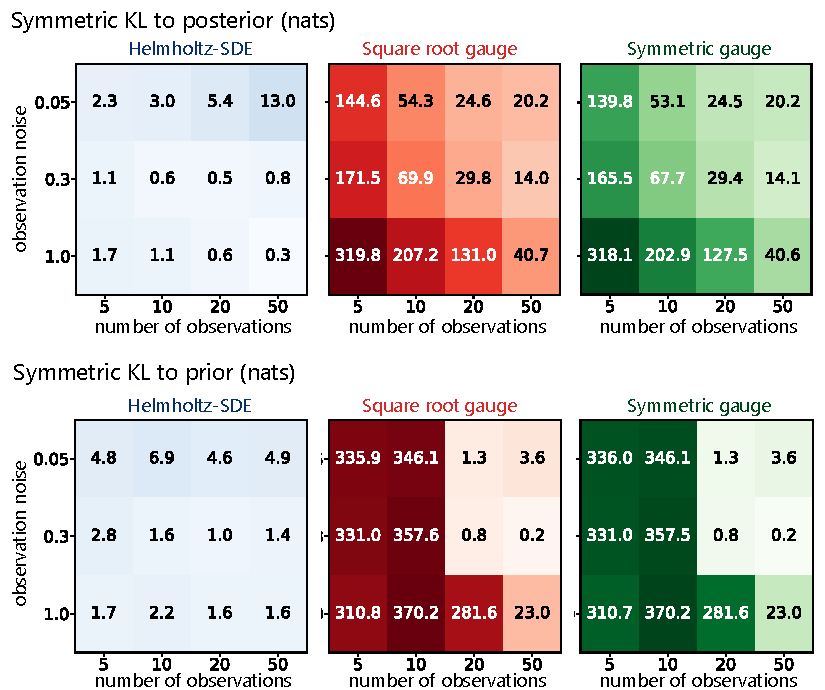
\includegraphics[width=0.9\textwidth]{figs/figs-spiral/results_2pi.pdf}
  \caption{OU spiral with $\omega = 2\pi$; top: symmetric KL to posterior; bottom: symmetric KL to prior.}
  \label{fig:spiral-2pi}
\end{figure}
\begin{figure}[!b]
  \centering
  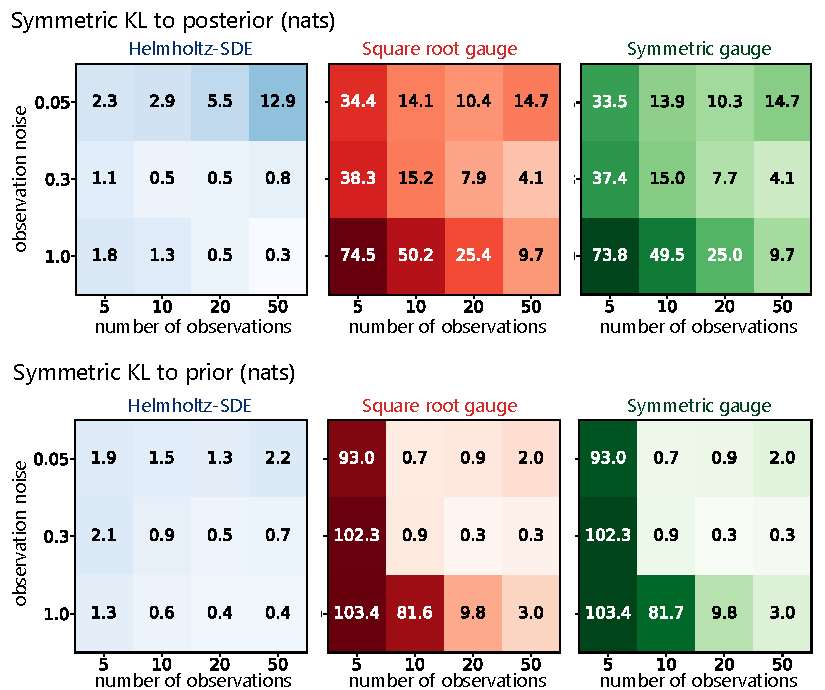
\includegraphics[width=0.9\textwidth]{figs/figs-spiral/results_pi.pdf}
  \caption{OU spiral  with $\omega = \pi$; top: symmetric KL to posterior; bottom: symmetric KL to prior.}
  \label{fig:spiral-pi}
\end{figure}

\clearpage
\begin{figure}[!t]
  \centering
  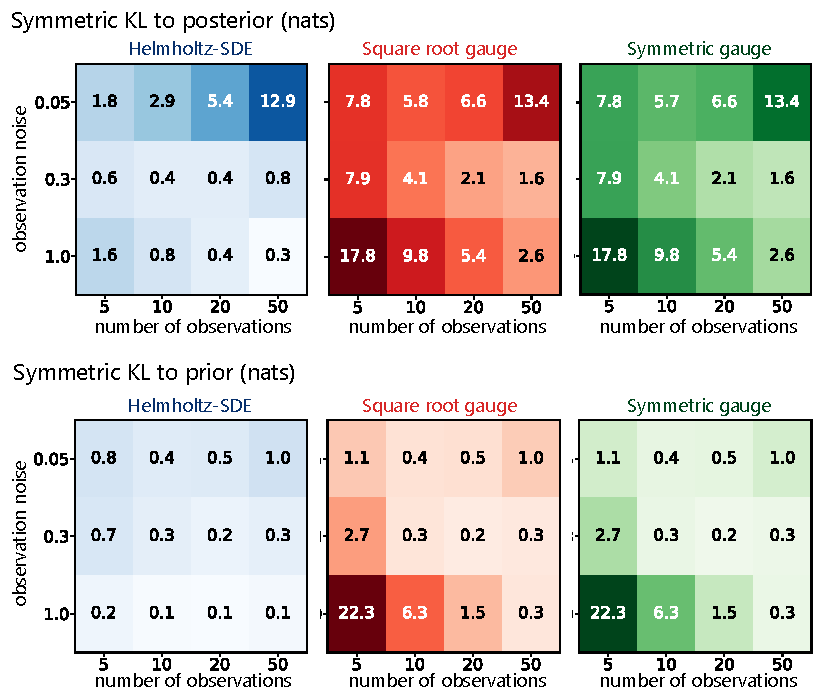
\includegraphics[width=0.9\textwidth]{figs/figs-spiral/results_pi2.pdf}
  \caption{OU spiral  with $\omega = \pi/2$; top: symmetric KL to posterior; bottom: symmetric KL to prior.}
  \label{fig:spiral-pi2}
\end{figure}
\begin{figure}[!b]
  \centering
  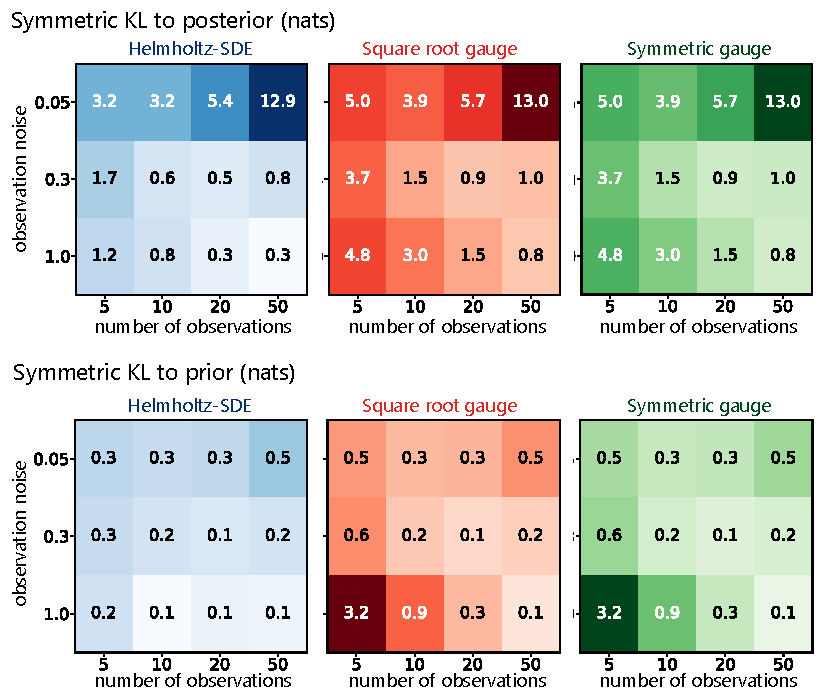
\includegraphics[width=0.9\textwidth]{figs/figs-spiral/results_pi4.pdf}
  \caption{OU spiral with $\omega = \pi/4$; top: symmetric KL to posterior; bottom: symmetric KL to prior.}
  \label{fig:spiral-pi4}
\end{figure}

\clearpage
\begin{figure}[!t]
  \centering
  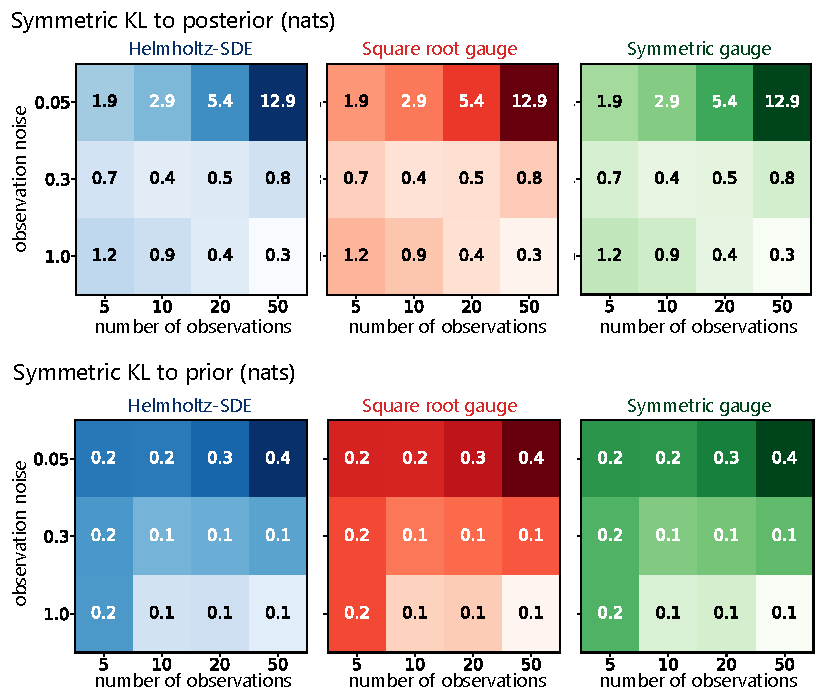
\includegraphics[width=0.9\textwidth]{figs/figs-spiral/results_zero.pdf}
  \caption{OU spiral  with $\omega = 0$; top: symmetric KL to posterior; bottom: symmetric KL to prior.}
  \label{fig:spiral-zero}
\end{figure}
\clearpage